\documentclass[11pt, a4paper, spanish]{article}

%%%%%%%%%% COMIENZO DEL PREAMBULO %%%%%%%%%%

%Info sobre este documento
\author{Martin Cammi}
\title{Trabajo Pr'actico de Ingenier'ia del software I}

%\usepackage{infostyle}                                                  % provee un look & feel similar a un documento Word
\usepackage[top=2.5cm, bottom=2.5cm, left=2.5cm, right=2.5cm]{geometry}  % m\'argenes
\usepackage[ansinew]{inputenc}                                           % permite que los acentos del estilo \'a\'e\'i\'o\'u salgan joya
\usepackage[spanish, activeacute]{babel}                                 % idioma espa\~{n}ol, acentos f\'aciles y deletreo de palabras
\usepackage{indentfirst}                                                 % permite indentar un parrafo a mano
\usepackage{caratula}                                                    % incluye caratula est\'andar
\usepackage{graphicx}                                                    % permite insertar gr\'aficos
\usepackage{color}                                                       % permite el uso de colores en el documento
\usepackage[pdfcreator={TexLive!, LaTeX2e con TeXnicCenter y la inteligencia de Jonathan ;-)},
			pdfauthor={Grupo 2"},
			pdftitle={Base de Datos - Trabajo practico: Campeonato Sudamericano de B\'asquet},
			pdfsubject={Trabajo Practico de Modelo de Entidad Relación},
			pdfkeywords={MER, MR},
			pdfstartview=FitH,            % Fits the width of the page to the window
			bookmarksnumbered,            % los bookmarks numerados se ven mejor...
			colorlinks,                   % links con bellos colores
			linkcolor=magenta]            % permite cambiar el color de los links
			{hyperref}                    % Permite jugar con algunas cosas que aparecer\'an en el PDF final
\usepackage{hyperref}
\usepackage{rotating}



%\selectlanguage{spanish}

\linespread{1.3}                    % interlineado equivalente al 1.5 l\'ineas de Word...
\pagestyle{myheadings}              %encabezado personalizable con \markboth{}{}
\markboth{}{Campeonato Sudamericano de B\'asquet. (Cammi, De Sousa, M\'endez, Serapio) }
\headsep = 30pt                     % separaci\'on entre encabezado y comienzo del p\'arrafo

%\addtolength{\oddsidemargin}{-2cm}	% configuracion IDEAL!!!
%\addtolength{\textwidth}{4cm}
%\addtolength{\textheight}{2cm}

% macro 'todo' para To-Do's
\def\todo#1{\textcolor{red}{#1}}

% Macro 'borde' para un texto con borde
\newsavebox{\fmbox}
\newenvironment{borde}[1]
{\begin{lrbox}{\fmbox}\begin{minipage}{#1}}
{\end{minipage}\end{lrbox}\fbox{\usebox{\fmbox}}\\[10pt]}

%%%%%%%%%% FIN DEL PREAMBULO %%%%%%%%%%

\begin{document}

\materia{Base de Datos}
\submateria{Segundo Cuatrimestre de 2012}
\titulo{Trabajo pr\'actico 1}
\subtitulo{Campeonato Sudamericano de B\'asquet.}
\grupo{Grupo 2}

\integrante{Cammi, Mart\'in}{676/02}{martincammi@gmail.com}
\integrante{De Sousa, Mariano}{389/08}{marian\_sabianaa@hotmail.com}
\integrante{M\'endez, Gonz\'alo}{843/04}{gemm83@hotmail.com}
\integrante{Serapio, Noelia}{871/03}{noeliaserapio@gmail.com}

\maketitle

\thispagestyle{empty}

\tableofcontents

\newpage

% Conviene poner las secciones como diferentes archivos,
% sobre todo cuando se trabaja en equipo.
% Es m\'as f\'acil para sincronizar mediante control de versiones.
%\input{Introducci\'on}


% BEGIN Ejemplos de uso

	%\section{Una secci\'on}
	%\label{sec:unaSeccion}
	%Hola! Soy una Secci\'on
	%	\subsection{Una subsecci\'on}
	%		Y yo soy una subsecci\'on!!!
	%		\subsubsection{Una subsubsecci\'on}
	%			Y yo soy una sub-subsecci\'on!!!
	%			\paragraph{Un p\'arrafo\\}
	%				Y yo soy un p\'arrafo, porque no hay mas sub-sub-sub-subsecciones!!!

	%\section{Otra secci\'on}
	%	Como pudimos ver en la secci\'on \ref{sec:unaSeccion}, esto es una demo de una referencia a una secci\'on.
	
	%	Tambi\'en podemos hacer referencia a la p\'agina de la secci\'on:\\[10pt]
	
		% Ejemplo de uso de un borde (falta pulir para que no tire un warning!)
	%	\begin{borde}{0.98\textwidth}
	%		En la p\'agina \pageref{sec:unaSeccion}, hay una secci\'on pilla...
	%	\end{borde}

% END Ejemplos de uso

\newpage
\section{Tecnolog\'ias utilizadas}
Hemos utilizado para la confecci\'on del trabajo pr\'actico el motor de base de datos Mysql

\newpage
	
\section{Modelo Entidad-Relacion}

	%\begin{sidewaysfigure}
	\begin{center}
		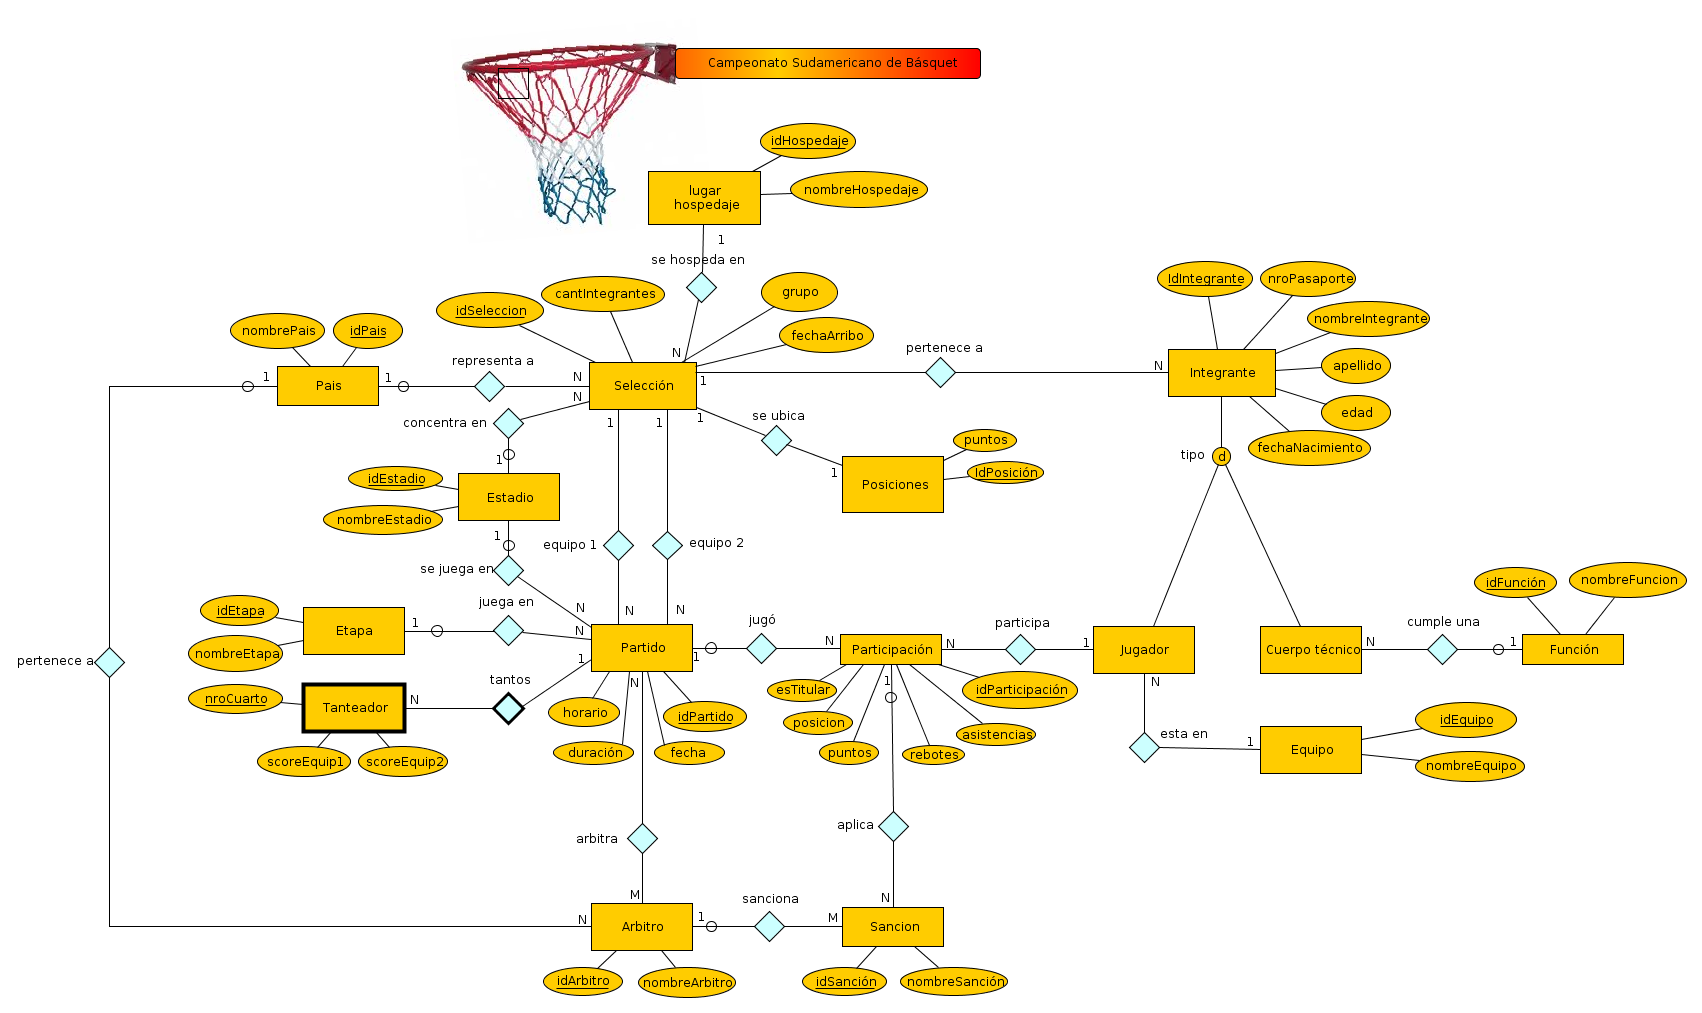
\includegraphics[scale=0.35]{diagramas/DiagramaMER.png}\\
	\end{center}
	%\end{sidewaysfigure}

\newpage 

\section{Modelo Logico Relacional}

\textbf{SELECCION}(idSeleccion, hospedaHospedaje, representaPais, concentraEstadio, ubicaPosicion, cantIntegrantes, fechaArribo, grupo)\\

PK = \{ (idSeleccion) \}\\
\indent{CC = \{ (idSeleccion) \}}\\
\indent{FK = \{ (hospedaHospedaje), (representaPais), (concentraEstadio), (ubicaPosicion) \}}\\

\noindent{ \textbf{References:}}

    SELECCION.hospedaHospedaje debe estar en LUGARHOSPEDAJE.idHospedaje\\
\indent{SELECCION.representaPais debe estar en PAIS.idPais}\\
\indent{SELECCION.concentraEstadio debe estar en ESTADIO.idEstadio}\\
\indent{SELECCION.ubicaPosicion debe estar en POSICION.idPosicion}\\

\indent{SELECCION.hospedaHospedaje no puede ser nulo}\\
\indent{SELECCION.representaPais no puede ser nulo}\\
\indent{SELECCION.concentraEstadio no puede ser nulo}\\
\indent{SELECCION.ubicaPosicion no puede ser nulo}\\


\noindent{ \textbf{Constraints:}}

\indent{SELECCION.grupo $==$ ``A`` no puede repetirse más de 4 veces.}\\
\indent{SELECCION.grupo $==$ ``B`` no puede repetirse más de 4 veces.}\\
\indent{SELECCION.grupo solo puede ser ``A`` o ``B``.}\\
\indent{SELECCION.fechaArribo <= PARTIDO.fecha.}\\
\indent{$\#$ SELECCION.cantIntegrantes debe ser igual a la cantidad de integrantes relacionados.}\\

\newpage 
\section{Supuestos asumidos}
Supuestos y asunciones.

\newpage 
\section{Dise\~{n}o f\'isico}
Detalle grafico o escrito de las tablas de mysql

\newpage 
\section{Restricciones adicionales al modelo}
Las 1000 restricciones que pusimos.

\newpage 
\section{Breakers}

Los breakers son sentencias de inserts dise\~{n}adas espec\'ificamente para poner a prueba las restricciones del modelo.
El archivo breakers.sql permite ejecutarlas y ver como todas ellas se verifican.

\newpage 
\section{Triggers y Store Procedures de restricciones}


\newpage 
\section{Datos de prueba}
Imagen de datos.sql y el fixture de los partidos con los puntajes

Todo el trabajo pr\'actico cuenta con 

\end{document}
